%%%%%%%%%%%%%%%%%%%%%%%%%%%%%%%%%%%%%%%%%%%%%%%
%
% Template for Bachelor degrees
% DISI - Dipartimento di Ingegneria e Scienza dell’Informazione
% DISI - Department of Information Engineering and Computer Science
%
% update 2020-08-30
%
% To generate pdf 
% pdflatex __filename__.tex
% bibtex __file_name__.aux
% pdflatex __file_name__.tex
% pdflatex __file_name__.tex
%
%%%%%%%%%%%%%%%%%%%%%%%%%%%%%%%%%%%%%%%%%%%%%%%

% !TEX root = surname_name_bachelorcourse_ay.tex

% 2 side format
\documentclass[epsfig,a4paper,11pt,titlepage,twoside,openany]{book}
\usepackage{epsfig}
\usepackage{plain}
\usepackage{setspace}
\usepackage[paperheight=29.7cm,paperwidth=21cm,outer=1.5cm,inner=2.5cm,top=2cm,bottom=2cm]{geometry} % layout setting
\usepackage{titlesec} % custom setup title of chanpter
% \usepackage{newtxtext,newtxmath} % times new roman

\usepackage{listings}
\usepackage{graphicx}
\usepackage{float}

\lstset{frame=tb,
  language=Bash,
  aboveskip=3mm,
  belowskip=3mm,
  showstringspaces=false,
  columns=flexible,
  basicstyle={\small\ttfamily},
  numbers=left,
  breaklines=true,
  breakatwhitespace=true,
  tabsize=3
}

%%%%%%%%%%%%%%
% support for accented letters
%
%\usepackage[latin1]{inputenc} % Windows;
\usepackage[utf8x]{inputenc} % Linux (unicode package is required);
%\usepackage[applemac]{inputenc} % Mac.

\singlespacing

% italian language
%\usepackage[italian]{babel}

\begin{document}

  % no page number
  \pagenumbering{gobble} 
  \pagestyle{plain}

\thispagestyle{empty}

\begin{center}
  \begin{figure}[h!]
    \centerline{
\psfig{file=marchio_unitrento_colore_it_202002.eps,width=0.6\textwidth}}
  \end{figure}

  \vspace{2 cm} 

  \LARGE{Department of Information Engineering and Computer Science\\}

  \vspace{1 cm} 
  \Large{Bachelor's Degree in\\
    Computer Science
    % Computer, Communication and Electronic Engineering
    % Information and Communications Engineering
    % Information and Business Organization Engineering
    % Electornics and Telecommunications Engineerign
  }

  \vspace{2 cm} 
  \Large\textsc{Final Dissertation\\} 
  \vspace{1 cm} 
  \Huge\textsc{Automated framework for IoT security testing\\}
  %\Large{\it{Sub-title (optional)}}


  \vspace{2 cm} 
  \begin{tabular*}{\textwidth}{ c @{\extracolsep{\fill}} c }
  \Large{Supervisor} & \Large{Student}\\
  \Large{Bruno Crispo}& \Large{Matteo Mariotti}\\
  \end{tabular*}

  \vspace{2 cm} 

  \Large{Academic year 2022/2023}
  
\end{center}



  \clearpage
 
%%%%%%%%%%%%%%%%%%%%%%%%%%%%%%%%%%%%%%%%%%%%%%%%%%%%%%%%%%%%%%%%%%%%%%%%%%
%%%%%%%%%%%%%%%%%%%%%%%%%%%%%%%%%%%%%%%%%%%%%%%%%%%%%%%%%%%%%%%%%%%%%%%%%%
%% Note
%%%%%%%%%%%%%%%%%%%%%%%%%%%%%%%%%%%%%%%%%%%%%%%%%%%%%%%%%%%%%%%%%%%%%%%%%%
%% Thanks/ Acknowledgements section is optional
%%%%%%%%%%%%%%%%%%%%%%%%%%%%%%%%%%%%%%%%%%%%%%%%%%%%%%%%%%%%%%%%%%%%%%%%%%
%%%%%%%%%%%%%%%%%%%%%%%%%%%%%%%%%%%%%%%%%%%%%%%%%%%%%%%%%%%%%%%%%%%%%%%%%%
  \thispagestyle{empty}

\begin{center}
  {\bf \Huge Acknowledgements}
\end{center}

\vspace{4cm}


\emph{
  ...thanks to... hello
}

  \clearpage
  \pagestyle{plain} % no heading, footer with centered page number

  
  % page number with Arabic format
  \mainmatter

%%%%%%%%%%%%%%%%%%%%%%%%%%%%%%%%%%%%%%%%%%%%%%%%%%%%%%%%%%%%%%%%%%%%%%%%%%
%%%%%%%%%%%%%%%%%%%%%%%%%%%%%%%%%%%%%%%%%%%%%%%%%%%%%%%%%%%%%%%%%%%%%%%%%%
%% Note
%%%%%%%%%%%%%%%%%%%%%%%%%%%%%%%%%%%%%%%%%%%%%%%%%%%%%%%%%%%%%%%%%%%%%%%%%%
%% The maximum number of pages is 30, including:
%%   index
%%   abstract
%%   chapters
%% Excluding:
%%   frontispiece
%%   acknowledgements 
%%   attachments
%%
%% For further details and updated rules, please check the guidelines.
%%%%%%%%%%%%%%%%%%%%%%%%%%%%%%%%%%%%%%%%%%%%%%%%%%%%%%%%%%%%%%%%%%%%%%%%%%
%%%%%%%%%%%%%%%%%%%%%%%%%%%%%%%%%%%%%%%%%%%%%%%%%%%%%%%%%%%%%%%%%%%%%%%%%%

    % index
    \tableofcontents
    \clearpage
    
    
          
    % group to define space between chapters
    \begingroup
      % no page break between chapters
      % override clear page commands
      \renewcommand{\cleardoublepage}{} 
      \renewcommand{\clearpage}{} 
      % override format of title chapter
      % from
      %   Chapter X
      %   Title
      % to
      %   X   Title
      
      \titleformat{\chapter}
        {\normalfont\Huge\bfseries}{\thechapter}{1em}{}
        
      \titlespacing*{\chapter}{0pt}{0.59in}{0.02in}
      \titlespacing*{\section}{0pt}{0.20in}{0.02in}
      \titlespacing*{\subsection}{0pt}{0.10in}{0.02in}
      
      % summary / abstract
      \chapter*{Abstract} % no number
\label{abtract}

\addcontentsline{toc}{chapter}{Abstract} % add to index

In the last few years, the security of IoT devices has become a major concern
in the field of Computer Science. In fact we are surrounded by always
new devices, such as cameras, smart speakers, and domotic devices in general,
that have become an integral part of our lives. \\
This means we are more and more exposed to attack that can compromise our
privacy and security. \\
The focus of this thesis is to automate the process of finding vulnerabilities
in such devices, by the means of finding the right tools and scripting the
various phases of the process. \\\\
This work will divided into two parts: a first more theoretical part, where
we will analyze the proposed tools and compare them to the ones used in previous works.
We will also analyze the scripts created to help the automation and explain their capabilities. \\
In a second, more practical part, we will test these tools on a real device,
focusing on the actions that have been successfully automated, and hence require
little to no user interaction. \\
\newpage
%%%%%%%%%%%%%%%%%%%%%%%%%%%%%%%%%%%%%%%%%%%%%%%%%%%%%%%%%%%%%%%%%%%%%%%%%%
%%%%%%%%%%%%%%%%%%%%%%%%%%%%%%%%%%%%%%%%%%%%%%%%%%%%%%%%%%%%%%%%%%%%%%%%%%
%% Note
%%%%%%%%%%%%%%%%%%%%%%%%%%%%%%%%%%%%%%%%%%%%%%%%%%%%%%%%%%%%%%%%%%%%%%%%%%
%% The abstract is a short summary of the work describing the target,
%% the subject of the thesis, the methodology and the techniques,
%% the data collection and elaboration, the explanation of the
%% reached results and the conclusion.
%% The abstract of the dissertation must have a maximum length of 3 pages
%% and must include the following information:
%%   context and motivation
%%   short summary of the main problem you have dealt with
%%   developed and /or used techniques 
%%   reached results, the personal contribution of the student has to be highlighted
%%%%%%%%%%%%%%%%%%%%%%%%%%%%%%%%%%%%%%%%%%%%%%%%%%%%%%%%%%%%%%%%%%%%%%%%%%
%%%%%%%%%%%%%%%%%%%%%%%%%%%%%%%%%%%%%%%%%%%%%%%%%%%%%%%%%%%%%%%%%%%%%%%%%%      
      
      \part{Tools}
      %%%%%%%%%%%%%%%%%%%%%%%%%%%%%%%%
      % chapters
      %
      % \input or \include
      %
      \chapter{Introduction}
In this part of the dissertation we will discuss the improvements over
previous works \cite{previouswork}, both in terms of alternative tools
with respect to the ones presented in that thesis, and in terms of additional
areas where we can search for vulnerabilities.\\
In particular we will discuss the following topics:
\begin{itemize}
    \item Gaining Wi-Fi access to the target network and exploring its weak points
    \item Attacks to the target network from the inside
    \item Attacks to the exported services of the target device, in particular web services
    \item An extension to the previous work, which allows to retrieve the memory
        image of the target device and analyze it offline
\end{itemize}
\newpage
      \chapter{Wi-Fi access}
In the thesis on which\cite{previouswork} this work is based it was suggested
to use the Fern wifi cracker\cite{fern} to gain access to the target newtwork.
Tis tool is basically a GUI for the aircrack-ng suite\cite{aircrack} and
exposes all the features of the command line tool. It can in fact perform
a lot of other attacks, aside from the WPA/WPA2 cracking, such as:
\begin{itemize}
    \item Automatic attacks on the access point
    \item MITM attacks
    \item Bruteforce attacks using protocols such as FTP, HTTP/HTTPS and TELNET
    \item Deauthentication, access point spoofing and replay attacks
\end{itemize}
Nevertheless, as the goal of this work is to automate the process, the command
line tool may prove to be more useful, as it can be easily integrated in a
script.\\
The Aircrack-ng suite is the most portable of the tools presented here, as it
can be used from virtually every operating system broadly used today, such as 
Windows, MacOS, a lot of Linux distributions and even from BSD operating systems.\\
There is also a Docker container for running it without installing it on the
main system. It can be installed using the right packaged version for the host OS
or by compiling it from source\cite{aircrack-git}.\\\\
Other tools that can be employed instead of aircrack-ng are:
\begin{itemize}
    \item Reaver\cite{reaver}: a tool that exploits a flaw in the WPS
        implementation of some routers using the WPS Pixie-Dust and other brute-force attacks
    \item Wifite\cite{wifite}: a python script that is a frontend for a lot of 
        tools, including aircrack-ng, reaver, cowpatty, pyrit, tshark, etc. It
        is therefore perfect to automate the process of vulnerability assessment
        of a wifi network
    \item Bully\cite{bully}: similar to Reaver
\end{itemize}
The suggested tool is Wifite, as it is the most complete and it is a frontend
to all other tools presented here. It is also a command line program, so it
can be easily used in a script and it's also very easy to use because of the
almost complete automation of the process. Unfortunately it needs many dependencies
to reach its full potential, but many of them are optional.
It can be downloaded using git in the following way:
\begin{lstlisting}[numbers=none]
    git clone https://github.com/derv82/wifite2.git
\end{lstlisting}
It can then be run opening the terminal in the cloned directory and running:
\begin{lstlisting}[numbers=none]
    sudo ./Wifite.py
\end{lstlisting}
\newpage
      \chapter{Memory analysis}
\section{Dump creation}
In this chapter well focus on memory analysis: a type of vulnerability assessment not part of the framework on which
this thesis is based. The goal will be to retrieve the memory dump of a running device
and analyze it to find out if it vulnerable.\\\\
We will assume the target device runs a Linux based operating system, because
in case of IoT devices this is the most common scenario. If the device has a
proprietary OS the analysis will be more difficult, but the same steps will apply
(dump creation, retrieve and analysis).\\
We also assume the attacker already has a working root shell on the device,
as all operations of memory read and kernel module loading are only allowed in
case of privileged access.\\\\
In order to do this we first have to extract the memory dump from the device
and put it in a file. This can be done using the dd command, present on all
Linux installations.\\ It can be used for example to copy the content of \textbf{/dev/mem}
calling it with the following syntax:
\begin{lstlisting}[numbers=none]
    dd if=/dev/mem of=memdump bs=1M count=1
\end{lstlisting}
This command will copy the specified number of blocks (count) of the specified
size (bs) to the specified output file.\\\\
Unfortunately we need a suitable device from which to extract the memory and \textbf{/dev/mem}
may have been configured to allow only a small amount of memory to be read:
this depends on the OS configuration so it's impossible to know it in advance.\\
This limit may be of 1Mb or 1Gb, depending on the architecture and configuration, but it's only
available since version 2.6.26 of the Linux kernel\cite{dev-mem-man} and only
if the kernel has been compiled with the \textbf{CONFIG\_STRICT\_DEVMEM} option.\\
On the x86 architecture it almost completely disallows memory access, allowing
only some memory addresses, such as memory mapped PCI devices, to be read.
The fact that the restriction is only available since a specific version may be an advantage for an attacker
because it means that older versions of the kernel (usually used on IoT devices) may not have it.\\\\
A similar device to textbf{/dev/mem} is \textbf{/dev/kmem}, which works the same 
way, but uses kernel virtual memory addresses instead of physical memory addresses.\\
Moreover it's only available if the kernel has been compiled with the \textbf{CONFIG\_DEVKMEM} option, so 
it's not always available and not a good choice for our purposes.\\\\
Another device from which we can obtain a memory dump is \textbf{/dev/fmem}\cite{dev-fmem}, which
can be created with the use of a kernel module. It allows to read the whole physical memory
without restrictions, but needs the installation of the kernel module and is not guaranteed to 
work with the specific kernel version or architecture. In fact it's not been updated
for a while, but this may not be a problem, because IoT devices rarely ship with the latest
kernel versions.\\
The last option that we'll analyze is the use of the \textbf{LiME} (Linux Memory Extractor)\cite{lime}.
It's the most advanced option, because it offers a lot of convenient
features that can help to retrieve the memory dump, with the downside (as before)
of needing the installation of a kernel module.\\
It can be used with the following syntax:
\begin{lstlisting}[numbers=none]
    insmod ./lime.ko "path=<outfile | tcp:<port>> format=<raw|padded|lime> [digest=<digest>] [dio=<0|1>]"
\end{lstlisting}
The module is able to:
\begin{itemize}
    \item Dump memory to a file or listen on a tcp port and send the memory dump to a remote host
    \item Use different formats for the memory dump
    \item Use different digest algorithms to verify the integrity of the memory dump 
\end{itemize}

\subsubsection{QEMU memory dump}
In case the attacker succeeded in emulating the device image with QUEMU (for example
using \textbf{FYRMADYNE}\cite{firmadyne}, as suggested in \cite{previouswork}), then it is possible
to obtain a memory dump of the emulated device.\\
This can be done with the \textbf{pmemsave} or the \textbf{dump-guest-memory} quemu commands.\\

\subsubsection{File retrieve}
Once we have created the memory dump we need to retrieve it from the device.\\
If LiMe was not used than it's possible to use the commands \textbf{netcat}\cite{netcat} or \textbf{scp}\cite{scp}
to upload the file to the attacker's machine.\\
As we assume the target device to be a Linux machine, scp will probably be installed
by default, whereas netcat will need to be installed.

\section{Analysis}
To analyze the dump file it's possible to use the \textbf{Volatility}\cite{volatility} framework, which is a collection
of python tools to analyze memory images and extract information from them.
We suggest using the original version, but there is also another one, more up to date, called \textbf{Volatility3}\cite{volatility3},
still in development.\\\\
It can be used for example to see open files and running processes at the time of the dump, but
has many capabilities, listed on the official documentation. Volatility supports
different file formats (raw, LiME, etc.) and different operating systems (Windows, Linux, etc.),
but for systems other than Windows you need to configure the right profile,
or even to write your own (in case there is no suitable one).\\\\
For Linux there are already some profiles available, but it's very likely that
an attacker will need to create his own ones, because of the huge variety of 
IoT devices. However the instructions can be found on the official documentation\cite{volatility-conf}.\\\\
Once the profile is configured it's possible to use the framework to analyze the dump file, to
retrieve all important information about the system. It's also possible to 
automate the process using the tool inside scripts, because it's a fully automated
framework.\\\\
\newpage
      \chapter{Scripts}
Here we will analyze the capabilities of the scripts developed for the project.\\
All the scripts are collected in a GitHub repository\cite{scripts-github}, so everyone
can find and use them and check their usage by reading the provided
documentation.
\section{Scan}
First of all we will analyze the script for the scanning and testing of the hosts on 
the network. It's a Bash script that uses \textbf{nmap} to discover hosts on the
network, search for open ports and run test script on those that are found.\\
If we run the script with the following option:
\begin{lstlisting}[numbers=none]
    scan -h
\end{lstlisting}
we will get all the options it can accept and the output will be the following:
\begin{lstlisting}[numbers=none]
    Usage: scan [OPTIONS]
        -u              perform udp scan
        -a              perform attack with default scripts
        -t              perform tcp scan
        -f              full scans
        -d              discovery mode (only -i and -o relevant)
        -v              scan for OS version
        -o FILENAME     redirect output to FILENAME
        -i IP           scan specified IP
        -m MODE         tcp scan mode
\end{lstlisting}
The \textbf{-d} option can be used to search for hosts on the network, and
only the \textbf{-i} and \textbf{-o} options will be relevant, all the others will
be discarded.\\
The \textbf{-i} option can be used to specify the IP address of the host to scan,
or of the network in case we are using the discovery mode (in which case we have to
specify the address using the CIDR notation). The \textbf{-o} option will cause 
all the outputs of the commands to be written also to that file, and not only to standard
output. In case we don't want to retain the output we can specify the \textbf{/dev/null} file.
If no file is specified it will default to "\textbf{output}".\\\\
We can pass the \textbf{-v} option to perform an OS scan on the specified
host, retrieving OS type and version.\\
The options \textbf{-t} or \textbf{-u}, which can be combined,
will perform a TCP or UDP scan respectively. The \textbf{-f} options will cause a full
scan to be performed, instead of only searching for the 1000 most common ports,
and it will affect bot UDP and TCP scans.
We can also specify the TCP scan mode to use with the \textbf{-m} option, in which
case it's not necessary to pass \textbf{-t}, because it is subsumed.\\
If the \textbf{-a} option is specified, the script will run the default nmap scripts
on the ports that are found open.\\\\
The script will also print every command executed and it's output, and it will
print what ports are found open before starting to, eventually, test them.
\section{New hosts discovery}
This script uses the \textbf{nmap} tool as before, to discover the newly connected
hosts on the network.\\
To obtain a help message from the script we can use the same syntax as before:
\begin{lstlisting}[numbers=none]
    find_hosts -h
\end{lstlisting}
and we will get the following output:
\begin{lstlisting}[numbers=none]
    Usage: find_hosts [OPTIONS]
    -h              print this help message
    -f FILE         get old IP addresses from FILE
    -i IP           scan specified IP
\end{lstlisting}
We see that we can use the \textbf{-i} option (required) to specify which network to scan,
passing an IP address in CIDR notation. The script will perform a first scan and
print the hosts that are found. It will then wait for the user to press enter,
after the new devices have been connected to the network, and it will perform
another scan, printing the IP addresses of the new hosts.\\\\
The process of waiting for the user to press enter can be avoided by passing
the \textbf{-f} option, which will cause the script to read the initial IP addresses
from a file (one address per line) and proceed directly to the second scan.
\section{Sniffing}
This script relies on the \textbf{ettercap}\cite{ettercap-home}\cite{ettercap-kali}\cite{ettercap-man} tool to sniff the packets between the two specified
hosts. It doesn't add much functionality, but it's useful to automate
and standardize the process, also simplifying its usage.\\
If we run the script with the following option:
\begin{lstlisting}[numbers=none]
    sniff -h
\end{lstlisting}
we will see the following output:
\begin{lstlisting}[numbers=none]
    Usage: sniff [OPTIONS]
    -h              print this help message
    -1 IP           specify first IP address
    -2 IP           specify second IP address
    -o FILE         write output to FILE
    -i IFACE        which interface to listen on
    -m MODE         what mode to use for mitm (default is arp)
\end{lstlisting}
We can use the \textbf{-1} and \textbf{-2} options to specify the IP addresses of the
two hosts we want to sniff (both are mandatory). The \textbf{-o} option can be used
to specify the file to which we want to write the output, and if it's not specified
it will default to "\textbf{output.pcap}".\\
The \textbf{-i} option can be used to specify the interface to listen on, and if it's
not specified it will default to "\textbf{wlo1}".\\
Finally, the \textbf{-m} option can be used to specify the mode to use for the mitm
attack, defaulting to \textbf{arp} if not specified.\\
This script, once started, will open the textual user interface of ettercap,
and will wait for the user to press \textbf{q} to quit, saving all packets
to the target output file.\\
\newpage
      \part{Scripts testing}
      \chapter{Device description}
The device we are going to use in this second part is produced by the same manufacturer
of the one used by Alessandro Bringhenti \cite{previouswork}, but is a different model, in particular
it is the Sricam SP017. It's a wireless IP camera, with night vision, motion detection
and two-way audio. It also integrates a microSD card slot and a wireless
access point, used to connect the phone for the first configuration.\\
As with the other model, at the bottom of the camera there the camera ID, also
encoded as a QR code, and the default password of the integrated access point.\\
The image of the device can be found in \textbf{Figure \ref{fig:sp017}}\\\\
We chose this device because of the cost (it can be bought on Amazon for 34€) and
because it has a two-way audio, so it could be more interesting to see which services
will be offered by the cam and test them.\\\\
To test the tools we will assume that the attacker is directly connected to the
same network of the attacker, so we will not cover the tolls presented to 
crack Wi-Fi passwords.\\\\\\\\
\begin{figure}[h]
    \centering
    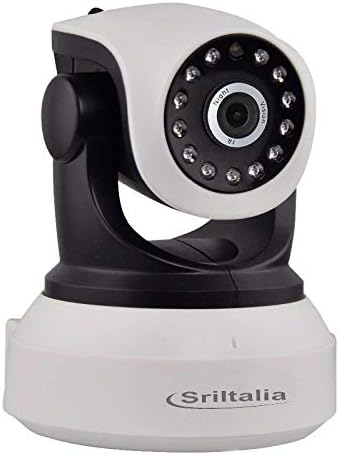
\includegraphics[scale=0.5]{cam.jpg}
    \caption{Sricam SP017}
    \label{fig:sp017}
\end{figure}
\newpage
      \chapter{Before device setup}
To bring up the device it's sufficient to connect it to the power supply, then it
will start emitting periodically a "beep" sound to indicate that it's ready to be configured.\\
Then we need to connect our phone and our computer to the device's wifi network:
the SSID is "IPC\_***" and the default password is "12345678".\\\\
After that we can start to scan the device using the script we wrote. First of all
we need to get the address IP of the device, and we can do that using the command:
\begin{lstlisting}[numbers=none]
    ip route
\end{lstlisting}
The output will be something like this:
\begin{lstlisting}[numbers=none]
    default via 192.168.66.1 dev wlo1 proto dhcp src 192.168.66.100 metric 20600 
    ...
\end{lstlisting}
So we can conclude that the IP address of the device is \textbf{192.168.66.100}.\\\\
Now we can start the script using the command:
\begin{lstlisting}[numbers=none]
    sudo ./scan -futav -o $FILENAME -i $IP
\end{lstlisting}
where \textbf{\$FILENAME} is the name of the file where we want to save the output
and \textbf{\$IP} is the IP address of the device. As previously
said this command requires to be run using root privileges
because of the use of the nmap command.\\\\
Regarding the OS version we got the following output:
\begin{lstlisting}[numbers=none]
    No exact OS matches for host (If you know what OS is running on it, see https://nmap.org/submit/ ).
\end{lstlisting}
from which we can understand that nmap was not able to identify the OS running
on the device.\\\\
We can also see that the device exposes various open ports:
\begin{lstlisting}[numbers=none]
    137/udp open netbios-ns
    138/udp open|filtered netbios-dgm
    139/tcp open netbios-ssn
    1716/tcp open xmsg
    1716/udp open|filtered xmsg
    41058/udp open|filtered unknown
    445/tcp open microsoft-ds
    445/tcp open netbios-ssn
    51225/udp open|filtered unknown
    5353/udp open zeroconf
    6566/tcp open sane-port
    6566/tcp open tcpwrapped
    8828/tcp open unknown
\end{lstlisting}
We can see that the UDP ports number 137 and 138 and the 139 TCP port are open,
which means that the device is exposing the \textbf{netbios} protocol, and the ports are used
respectively to provide name lookup (137), the datagram service (138) and the session
service (139) \cite{netbios-ws}\cite{netbios-smb}.\\
We can also see that the port 1716 is open for both TCP and UDP (although filtered), and exposes
\textbf{xmsg} services, used to share information via XML documents.\\\\
Then we have port 445 (both UDP and TCP) which is associated with \textbf{SMB}:
a protocol developed by Microsoft to share files between machines over network.\\
The port for the \textbf{zeroconf} service is used to dynamically configure the
hosts on the network \cite{zeroconf}, and \textbf{sane-port} is a protocol used
to share scanner devices over network. The latter is also reported as a tcpwrapped port, which means
that the port is protected by TCP Wrappers, an ACL system used to filter incoming packages
using rules (such as allow only some hosts) in a similar way to firewalls. \\\\
Then we also have two ports that are unknown, because they are not standard, therefore we don't know what services
are associated with them.\\\\
Then we have the output associated with the scripts run by nmap, which reports the following:
\begin{lstlisting}[numbers=none]
    ...
    PORT    STATE SERVICE
    139/tcp open  netbios-ssn

    Host script results:
    |_nbstat: NetBIOS name: , NetBIOS user: <unknown>, NetBIOS MAC: <unknown> (unknown)
    | smb2-security-mode: 
    |   3:1:1: 
    |_    Message signing enabled but not required
    | smb2-time: 
    |   date: 2023-08-14T14:36:09
    |_  start_date: N/A

    ...
    PORT    STATE SERVICE
    445/tcp open  microsoft-ds

    Host script results:
    | smb2-time: 
    |   date: 2023-08-14T14:36:51
    |_  start_date: N/A
    | smb2-security-mode: 
    |   3:1:1: 
    |_    Message signing enabled but not required
    |_clock-skew: -1s
    |_nbstat: NetBIOS name: , NetBIOS user: <unknown>, NetBIOS MAC: <unknown> (unknown)

    ...
\end{lstlisting}
This output is generated by the \textbf{smb2-security-mode} script \cite{smb-script},
which complains about the fact that the message signing is enabled but not required,
and this could lead to security issues.\\\\
Then we have the output of the \textbf{nbstat} script \cite{nbstat}, which
unfortunately doesn't find any hostname and is not able to retrieve the netbios user or the MAC address.
\newpage
      \chapter{After setup}

\section{Setup}
To setup the camera it is sufficient to connect the phone to the camera wifi
and add the device to the app. The app will automatically connect to the camera
and we will be able to configure the camera to connect to the local wifi.
In case the camera has been connected using the ethernet cable, it is
sufficient to add it to the app using the QR code on the back of the camera.\\\\
After having configured the camera we can use the script created to list new hosts
in a network to find the IP addresses of the camera and the phone.\\
It can be run using this command:
\begin{lstlisting}[numbers=none]
    sudo ./find_hosts -i 192.168.200.223/24
\end{lstlisting}
where the IP address is the one of the local network (which
can be found using the \textbf{ifconfig} command).\\
An example of the output of the script is the following:
\begin{lstlisting}[numbers=none]
    ...
    192.168.200.237
\end{lstlisting}
We can confirm this is the IP address of the camera by checking on
the app. The address of the phone can be found in the same manner and in our case
it was \textbf{192.168.200.226}.\\
\section{Scanning}
We can now repeat the scan of the camera to see which ports are open, now that the
configuration has changed.\\
We can run the script using the same command as before command:
\begin{lstlisting}[numbers=none]
    sudo ./scan -futav -o $FILENAME -i 192.168.200.237
\end{lstlisting}
Strangely enough, the script did not recognize the camera operating system
and MAC address the first time it was run.\\
But the second time correctly gave the following output:
\begin{lstlisting}[numbers=none]
    ... 
    MAC Address: E0:51:D8:ED:73:85 (China Dragon Technology Limited)
    Device type: general purpose
    Running: Linux 2.6.X|3.X
    OS CPE: cpe:/o:linux:linux_kernel:2.6 cpe:/o:linux:linux_kernel:3
    OS details: Linux 2.6.32 - 3.5
    Uptime guess: 0.004 days (since Tue Aug 22 17:34:17 2023)
    Network Distance: 1 hop
    ... 
\end{lstlisting}
We can see that it runs a Linux kernel between 2.6.32 and 3.5, so it's not 
the latest version, and this may lead to some security issues.\\\\
We found that the open ports are the following:
\begin{lstlisting}[numbers=none]
    1300/tcp open h323hostcallsc
    19096/udp open|filtered unknown
    3702/udp open|filtered ws-discovery
    443/tcp open ssl/https
    49167/udp open|filtered unknown
    80/tcp open http
    8000/udp open|filtered irdmi
    843/tcp open unknown
\end{lstlisting}
The script also complained about two services being unrecognized, despite having
returned data during the first scan.\\
We can see that the ports associated to the SMB protocol are not open anymore,
but we have some new ports, such as the 80 and 443 over TCP, which are used by \textbf{HTTP}
and \textbf{HTTPS}, probably for the administration interface of the camera.\\\\
Another interesting port is the number 1300, which is used by the \textbf{H.323} protocol,
which is used to send and receive audio and video over the network \cite{h323}.\\
Other open ports are the ones associated with
\textbf{ws-discovery}, a protocol to search for web services on
a network \cite{ws-discovery}, and \textbf{irdmi}, a protocol developed
by Intel that provides a remote desktop management interface for
the device.\\\\
During the test phase of those ports, we got the following output:
\begin{lstlisting}[numbers=none]
    ... 

    PORT    STATE SERVICE
    443/tcp open  https
    | ssl-cert: Subject: commonName=localhost/organizationName=Example.com/stateOrProvinceName=Washington/countryName=US
    | Issuer: commonName=localhost/organizationName=Example.com/stateOrProvinceName=Washington/countryName=US
    | Public Key type: rsa
    | Public Key bits: 2048
    | Signature Algorithm: sha256WithRSAEncryption
    | Not valid before: 2015-10-29T00:57:15
    | Not valid after:  2025-10-26T00:57:15
    | MD5:   2b31:8848:da07:3366:8eba:ecf3:9c96:0be3
    |_SHA-1: 48f0:92d1:bc58:b700:b956:2fb3:5819:efee:c4e8:8eab

    ... 

    PORT   STATE SERVICE
    80/tcp open  http
    |_http-favicon: Unknown favicon MD5: 761B3CBCC87F3F8BE5FCF40C779E98B9
    | http-methods: 
    |_  Supported Methods: GET HEAD POST
    | http-title: index
    |_Requested resource was http://192.168.200.237/index.html

    ... 
\end{lstlisting}
The only useful information we can get from this output is what
HTTP methods are allowed by the server, which are \textbf{GET}, \textbf{HEAD} and \textbf{POST}, 
and some information about the SSL certificate used by the HTTPS server.\\
\section{Packet sniffing}
We can now try to sniff the traffic between the camera and the router and between
the phone and the router.\\
We can use the script created to sniff the traffic and save it to a file, and
analyze later the pcap using Wireshark.\\
We can run the script using the following command:
\begin{lstlisting}[numbers=none]
    sudo ./sniff -1 192.168.200.226 -2 192.168.200.1 -i wlo1
\end{lstlisting}
to start the sniffing process for the camera. Unfortunately, the analysis of the
pcap file did not give any useful information, so we were not able to get the source
for the firmware updates of the camera and we could not analyze it further. 
\newpage
      
      
    \endgroup


    % bibliography - bibtex format
    %
    % add chapter to index
    \addcontentsline{toc}{chapter}{Bibliography}
    % alphabetical order of authors
    \bibliographystyle{plain}
    \bibliography{biblio}
%%%%%%%%%%%%%%%%%%%%%%%%%%%%%%%%%%%%%%%%%%%%%%%%%%%%%%%%%%%%%%%%%%%%%%%%%%
%%%%%%%%%%%%%%%%%%%%%%%%%%%%%%%%%%%%%%%%%%%%%%%%%%%%%%%%%%%%%%%%%%%%%%%%%%
%% Nota
%%%%%%%%%%%%%%%%%%%%%%%%%%%%%%%%%%%%%%%%%%%%%%%%%%%%%%%%%%%%%%%%%%%%%%%%%%
%% In the bibliography, all the sources consulted for the dissertation 
%% have to be cited and listed in alphabetical order by the 
%% first author's surname.
%%
%% According to the source material, the quotation has to be as follows:
%%
%% BOOKS
%% Surname and initial/s of the name/s of the author/s, date of edition,
%% publishing house and (if applicable) number of edition.
%% 
%% JOURNAL ARTICLES 
%% Surname and initial/s of the first name/s of the author/s,
%% title of the article, name of the journal, volume number, issue number
%% and page numbers.
%% 
%% CONFERENCE PAPERS
%% Surname and initial/s of the name/s of the author/s,
%% year of the conference, title of the article, name of the conference,
%% place of the conference, conference dates, page numbers.
%% 
%% CITING WEB RESOURCES
%% The consulted webpages have to be listed in alphabetical order. 
%% It is necessary to:
%%   - Copy the specific URL (the web address) of the consulted webpage
%%   - If available, indicate the surname and first name of the author/s,
%%     the title and subtitle of the text
%%   - If available, indicate the last date you retrieved the webpage
%%     (day/month/year).   
%%%%%%%%%%%%%%%%%%%%%%%%%%%%%%%%%%%%%%%%%%%%%%%%%%%%%%%%%%%%%%%%%%%%%%%%%%
%%%%%%%%%%%%%%%%%%%%%%%%%%%%%%%%%%%%%%%%%%%%%%%%%%%%%%%%%%%%%%%%%%%%%%%%%%
    

    \titleformat{\chapter}
        {\normalfont\Huge\bfseries}{Appendix \thechapter}{1em}{}
    % Appendix / attachment section - optional
    \appendix
    \chapter{Title first appendix}

Lorem ipsum dolor sit amet, consectetur adipiscing elit. Donec sed nunc orci. Aliquam nec nisl vitae sapien pulvinar dictum quis non urna. Suspendisse at dui a erat aliquam vestibulum. Quisque ultrices pellentesque pellentesque. Pellentesque egestas quam sed blandit tempus. Sed congue nec risus posuere euismod. Maecenas ut lacus id mauris sagittis egestas a eu dui. Class aptent taciti sociosqu ad litora torquent per conubia nostra, per inceptos himenaeos. Pellentesque at ultrices tellus. Ut eu purus eget sem iaculis ultricies sed non lorem. Curabitur gravida dui eget ex vestibulum venenatis. Phasellus gravida tellus velit, non eleifend justo lobortis eget. 

\section{Title}
Lorem ipsum dolor sit amet, consectetur adipiscing elit. Donec sed nunc orci. Aliquam nec nisl vitae sapien pulvinar dictum quis non urna. Suspendisse at dui a erat aliquam vestibulum. Quisque ultrices pellentesque pellentesque. Pellentesque egestas quam sed blandit tempus. Sed congue nec risus posuere euismod. Maecenas ut lacus id mauris sagittis egestas a eu dui. Class aptent taciti sociosqu ad litora torquent per conubia nostra, per inceptos himenaeos. Pellentesque at ultrices tellus. Ut eu purus eget sem iaculis ultricies sed non lorem. Curabitur gravida dui eget ex vestibulum venenatis. Phasellus gravida tellus velit, non eleifend justo lobortis eget. 

\subsection{Sub-title}
Lorem ipsum dolor sit amet, consectetur adipiscing elit. Donec sed nunc orci. Aliquam nec nisl vitae sapien pulvinar dictum quis non urna. Suspendisse at dui a erat aliquam vestibulum. Quisque ultrices pellentesque pellentesque. Pellentesque egestas quam sed blandit tempus. Sed congue nec risus posuere euismod. Maecenas ut lacus id mauris sagittis egestas a eu dui. Class aptent taciti sociosqu ad litora torquent per conubia nostra, per inceptos himenaeos. Pellentesque at ultrices tellus. Ut eu purus eget sem iaculis ultricies sed non lorem. Curabitur gravida dui eget ex vestibulum venenatis. Phasellus gravida tellus velit, non eleifend justo lobortis eget. 


\chapter{Title first appendix}

Lorem ipsum dolor sit amet, consectetur adipiscing elit. Donec sed nunc orci. Aliquam nec nisl vitae sapien pulvinar dictum quis non urna. Suspendisse at dui a erat aliquam vestibulum. Quisque ultrices pellentesque pellentesque. Pellentesque egestas quam sed blandit tempus. Sed congue nec risus posuere euismod. Maecenas ut lacus id mauris sagittis egestas a eu dui. Class aptent taciti sociosqu ad litora torquent per conubia nostra, per inceptos himenaeos. Pellentesque at ultrices tellus. Ut eu purus eget sem iaculis ultricies sed non lorem. Curabitur gravida dui eget ex vestibulum venenatis. Phasellus gravida tellus velit, non eleifend justo lobortis eget. 

\section{Title}
Lorem ipsum dolor sit amet, consectetur adipiscing elit. Donec sed nunc orci. Aliquam nec nisl vitae sapien pulvinar dictum quis non urna. Suspendisse at dui a erat aliquam vestibulum. Quisque ultrices pellentesque pellentesque. Pellentesque egestas quam sed blandit tempus. Sed congue nec risus posuere euismod. Maecenas ut lacus id mauris sagittis egestas a eu dui. Class aptent taciti sociosqu ad litora torquent per conubia nostra, per inceptos himenaeos. Pellentesque at ultrices tellus. Ut eu purus eget sem iaculis ultricies sed non lorem. Curabitur gravida dui eget ex vestibulum venenatis. Phasellus gravida tellus velit, non eleifend justo lobortis eget. 

\subsection{Sub-title}
Lorem ipsum dolor sit amet, consectetur adipiscing elit. Donec sed nunc orci. Aliquam nec nisl vitae sapien pulvinar dictum quis non urna. Suspendisse at dui a erat aliquam vestibulum. Quisque ultrices pellentesque pellentesque. Pellentesque egestas quam sed blandit tempus. Sed congue nec risus posuere euismod. Maecenas ut lacus id mauris sagittis egestas a eu dui. Class aptent taciti sociosqu ad litora torquent per conubia nostra, per inceptos himenaeos. Pellentesque at ultrices tellus. Ut eu purus eget sem iaculis ultricies sed non lorem. Curabitur gravida dui eget ex vestibulum venenatis. Phasellus gravida tellus velit, non eleifend justo lobortis eget. 




\end{document}
